% Template last modified by Jake Hart; please contact course staff if you have any questions regarding using this template

\documentclass{METUHW} % You must have the cisXXX .cls file in your project or working directory (i.e. the same directory as this document) 
\HWno{1} % Enter the number of the homework you are working on
\HWcourse{EE313} % Enter the course department and number here
\HWpartner{Özgür Gülsuna} % If your class allows group work, put your partners here
\usepackage{amsmath}
\usepackage{calc}
\usepackage{xcolor}\pagecolor{white}
\usepackage[linguistics]{forest}
\usepackage{listings}[language=matlab]
\usepackage{listings}
\usepackage{color}
\usepackage{xcolor}
\usepackage[colorinlistoftodos]{todonotes}
\usepackage{float}
\usepackage{circuitikz}
\usepackage{ragged2e}
\usepackage{steinmetz}


%includes for tikz
\usepackage{physics}
\usepackage{amsmath}
\usepackage{tikz}
\usepackage{mathdots}
\usepackage{yhmath}
\usepackage{cancel}
\usepackage{color}
\usepackage{siunitx}
\usepackage{array}
\usepackage{multirow}
\usepackage{amssymb}
\usepackage{gensymb}
\usepackage{tabularx}
\usepackage{extarrows}
\usepackage{booktabs}
\usetikzlibrary{fadings}
\usetikzlibrary{patterns}
\usetikzlibrary{shadows.blur}
\usetikzlibrary{shapes}


\usepackage{physics}
\usepackage{amsmath}
\usepackage{tikz}
\usepackage{mathdots}
\usepackage{yhmath}
\usepackage{cancel}
\usepackage{color}
\usepackage{siunitx}
\usepackage{array}
\usepackage{multirow}
\usepackage{amssymb}
\usepackage{gensymb}
\usepackage{tabularx}
\usepackage{extarrows}
\usepackage{booktabs}
\usetikzlibrary{fadings}
\usetikzlibrary{patterns}
\usetikzlibrary{shadows.blur}
\usetikzlibrary{shapes}




\restylefloat{table}

\definecolor{codegreen}{rgb}{0,0.5,0.5}
\definecolor{codegray}{rgb}{0.5,0.5,0.5}
\definecolor{codepurple}{rgb}{0.6,0.1,0.1}
\definecolor{backcolour}{rgb}{0.95,0.95,0.95}

\lstdefinestyle{mystyle}{
    backgroundcolor=\color{backcolour},   
    commentstyle=\color{codegreen},
    keywordstyle=\color{magenta},
    numberstyle=\tiny\color{codegray},
    stringstyle=\color{codepurple},
    basicstyle=\ttfamily\footnotesize,
    breakatwhitespace=false,         
    breaklines=true,                 
    captionpos=b,                    
    keepspaces=true,                 
    numbers=false,                    
    numbersep=5pt,                  
    showspaces=false,                
    showstringspaces=false,
    showtabs=false,                  
    tabsize=2
}

\lstset{style=mystyle}

\newcommand*{\CenterVdots}{\makebox[\widthof{(0,0),}][c]{\vdots}}


\begin{document}

\title{{%   <-- starts a group
\vspace{-3cm}
\scriptsize
\normalsize
\textbf{EE313 ANALOG ELECTRONICS LABORATORY \\ \small TERM PROJECT}\\
\large\\
}%   <-- ends that group

\textbf{
PROPOSAL REPORT\\
}
\small
Design of a Micro-Air Conditioner\\
\medskip
\medskip
\medskip
\small

Özgür Gülsuna 2307668 \hfill 16.01.2022\\
\raggedright
Işık Emir Altunkol 2442408 \hfill Time Spent: 12 hours

}

\author{ }
\date{ }
\maketitle


\vspace{-4em}

\justifying

    To design an air conditioning system, we need to have a sensing unit, display unit, control unit, and an operation unit. In this document, we will explain our approach to implement those functioning units one by one. \\
\medskip

\textbf{ \normalsize Sensing Unit}\\
\fontsğze
    Sensing unit is a simple unit consisting of a temperature sensor and its amplifier. For the actual sensor we are going to use LM35. It will give a voltage output which has a linear relation with the temperature in the specified range. Some of the other features of this sensor are, 4-30 V operation range and 0.5°C accuracy. Amplifier at the output of the temperature sensor will enable us to isolate the different parts of the circuit which ensure its reliability and it will help us to scale the reading to a more useful range. We will place the sensor close enough to the heating and cooling elements so that we can change the temperature at the desired rate.\\

\medskip

\textbf{ \normalsize Display Unit}\\
    Display unit consists of two sets of RGB LEDs (red-green-blue light emitting diodes) in common anode configuration - one for displaying the set value, and the other for displaying the measured room temperature. We wanted to separate the LEDs to better visualize the operation of the system. As described in the project, we have a color bar indicating the temperatures. To achieve the same output we need to create three different signals for each LED.  Required signal for each color is shown in Figure 1. Series of operational amplifier structures will be used to generate the aforementioned signal. When it comes to driving the LEDs we will utilize bipolar junction transistors (BJTs). These semiconductor devices enable us to control the current of the individual LEDs which corresponds to their brightness. The selected topology is a common emitter amplifier. This structure is also named as  transconductance amplifier, which means that an input voltage produces an output current.


\begin{figure}[H]
\centering
\includegraphics[scale=0.30]{figure/fig1.png}\\
\centering
Figure 1. LED driving signals for each color.
\end{figure}


\textbf{ \normalsize Control Unit}\\
    Control unit has the highest complexity among others. It will have several parts for handling various tasks. First of all, it will take input from two different sources. First one will be the amplified output voltage of the temperature sensor. Second one will be the reading from the potentiometer. This unit will generate outputs for two different elements, heating and cooling respectively. We decided to implement a PID (proportional integral derivative) controller for this task, which is a controller with feedback. This way we can control the elements in an analogous fashion. We will take the input from the potentiometer as the set point and the amplified LM35 output as the process variable. The PID implementation will be done with operational amplifier configurations as shown in Figure 2. For op-amp selection, we will go with LM358 dual channel op-amps. They are cheap, reliable and suitable for the control unit. Also a dead-band is constructed at the end of this stage.


\centering



\tikzset{every picture/.style={line width=0.75pt}} %set default line width to 0.75pt        

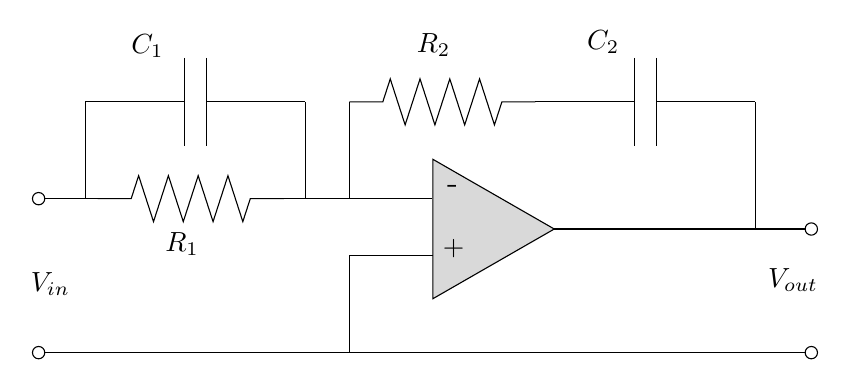
\begin{tikzpicture}[x=0.75pt,y=0.75pt,yscale=-1,xscale=1]
%uncomment if require: \path (0,208); %set diagram left start at 0, and has height of 208

%Shape: Resistor [id:dp8858278922494136] 
\draw   (174.26,88.32) -- (190.4,88.32) -- (193.99,77.25) -- (201.16,99.39) -- (208.33,77.25) -- (215.5,99.39) -- (222.68,77.25) -- (229.85,99.39) -- (237.02,77.25) -- (244.19,99.39) -- (247.78,88.32) -- (263.92,88.32) ;
%Shape: Capacitor [id:dp03371552137820011] 
\draw   (168.33,41.69) -- (216.02,41.69) (226.61,20.5) -- (226.61,62.89) (216.02,20.5) -- (216.02,62.89) (226.61,41.69) -- (274.3,41.69) ;
%Shape: Triangle [id:dp98497243420744] 
\draw  [fill={rgb, 255:red, 217; green, 217; blue, 217 }  ,fill opacity=1 ] (394.24,102.94) -- (335.76,136.52) -- (335.76,69.35) -- cycle ;
%Straight Lines [id:da3971318773795933] 
\draw    (168.33,41.69) -- (168.33,88.32) ;
%Straight Lines [id:da3049997475460431] 
\draw    (274.3,41.69) -- (274.3,88.32) ;
%Straight Lines [id:da7159809408880349] 
\draw    (274.3,88.32) -- (335.34,88.32) ;
%Straight Lines [id:da9186521041305018] 
\draw    (174.26,88.32) -- (168.33,88.32) ;
%Straight Lines [id:da0908787872310326] 
\draw    (263.92,88.32) -- (274.3,88.32) ;
%Shape: Resistor [id:dp13518795960649532] 
\draw   (295.49,41.69) -- (311.63,41.69) -- (315.22,30.62) -- (322.39,52.77) -- (329.56,30.62) -- (336.73,52.77) -- (343.91,30.62) -- (351.08,52.77) -- (358.25,30.62) -- (365.42,52.77) -- (369.01,41.69) -- (385.15,41.69) ;
%Straight Lines [id:da3878971923579282] 
\draw    (295.49,41.69) -- (295.49,88.32) ;
%Shape: Capacitor [id:dp1987350161026391] 
\draw   (385.15,41.69) -- (432.83,41.69) (443.43,20.5) -- (443.43,62.89) (432.83,20.5) -- (432.83,62.89) (443.43,41.69) -- (491.12,41.69) ;
%Straight Lines [id:da7857458487620923] 
\draw    (394.24,102.94) -- (515.13,102.94) ;
%Straight Lines [id:da3195712557469328] 
\draw    (491.12,41.69) -- (491.12,102.94) ;
%Straight Lines [id:da9218474418090266] 
\draw    (295.49,115.87) -- (295.49,162.5) ;
%Straight Lines [id:da3520350954534184] 
\draw    (295.49,115.87) -- (335.88,115.87) ;
%Straight Lines [id:da9046341306409746] 
\draw    (295.49,162.5) -- (148.77,162.5) ;
%Straight Lines [id:da6420173241490861] 
\draw    (515.13,162.5) -- (295.49,162.5) ;
%Straight Lines [id:da18257571009246387] 
\draw    (168.33,88.32) -- (148.77,88.32) ;
%Flowchart: Connector [id:dp0488086244709538] 
\draw   (142.84,88.32) .. controls (142.84,86.68) and (144.17,85.35) .. (145.8,85.35) .. controls (147.44,85.35) and (148.77,86.68) .. (148.77,88.32) .. controls (148.77,89.96) and (147.44,91.29) .. (145.8,91.29) .. controls (144.17,91.29) and (142.84,89.96) .. (142.84,88.32) -- cycle ;
%Flowchart: Connector [id:dp7782162243873112] 
\draw   (142.84,162.5) .. controls (142.84,160.86) and (144.17,159.53) .. (145.8,159.53) .. controls (147.44,159.53) and (148.77,160.86) .. (148.77,162.5) .. controls (148.77,164.14) and (147.44,165.47) .. (145.8,165.47) .. controls (144.17,165.47) and (142.84,164.14) .. (142.84,162.5) -- cycle ;
%Flowchart: Connector [id:dp7350444455171572] 
\draw   (515.13,162.5) .. controls (515.13,160.86) and (516.45,159.53) .. (518.09,159.53) .. controls (519.73,159.53) and (521.06,160.86) .. (521.06,162.5) .. controls (521.06,164.14) and (519.73,165.47) .. (518.09,165.47) .. controls (516.45,165.47) and (515.13,164.14) .. (515.13,162.5) -- cycle ;
%Flowchart: Connector [id:dp4930242403173162] 
\draw   (515.13,102.94) .. controls (515.13,101.3) and (516.45,99.97) .. (518.09,99.97) .. controls (519.73,99.97) and (521.06,101.3) .. (521.06,102.94) .. controls (521.06,104.58) and (519.73,105.9) .. (518.09,105.9) .. controls (516.45,105.9) and (515.13,104.58) .. (515.13,102.94) -- cycle ;

% Text Node
\draw (339.35,106.62) node [anchor=north west][inner sep=0.75pt]   [align=left] {+};
% Text Node
\draw (341.37,77.77) node [anchor=north west][inner sep=0.75pt]   [align=left] {{\large -}};
% Text Node
\draw (205.6,103.2) node [anchor=north west][inner sep=0.75pt]    {$R_{1}$};
% Text Node
\draw (326.8,7.4) node [anchor=north west][inner sep=0.75pt]    {$R_{2}$};
% Text Node
\draw (189.2,8) node [anchor=north west][inner sep=0.75pt]    {$C_{1}$};
% Text Node
\draw (408.8,6.2) node [anchor=north west][inner sep=0.75pt]    {$C_{2}$};
% Text Node
\draw (140.8,122.8) node [anchor=north west][inner sep=0.75pt]    {$V_{in}$};
% Text Node
\draw (496,120.8) node [anchor=north west][inner sep=0.75pt]    {$V_{out}$};


\end{tikzpicture}

\\

\centering
Figure 2. PID controller implemented with single operational amplifier.\\

\medskip

\raggedright

\justifying

\textbf{ \normalsize Operation Unit}\\
    Operation unit is sort of a driver unit. In this section, output of the control unit is picked up and converted into pulse width modulation (PWM) signals so that our elements can be controlled more accurately. An oscillator will be implemented in this section to generate the PWM clock for the elements. This single clock will be utilized by both of the comparator blocks, which means that their frequency will be the same. Basically the triangle oscillator is compared with control signals to generate desired PWM signals for each output. Later these signals are fed onto mosfet bridges to adjust the power given to each element. The heating element is selected as a piece of nickel-chromium wire. The heating wire will be wrapped around our temperature sensor without touching to ensure more of the power is transferred onto the sensor. The resistance value for the wire will be chosen such that at most it will dissipate 10 watts of power. For cooling we will use a 12 V computer fan, which takes direct current voltage for an input. The power consumption of the selected fan is around 2 watts. Preliminary experiments showed that these power ratings will be fairly enough.\\
    
\medskip

\textbf{ \normalsize Mechanical Design}\\
Mechanical construction of the system is decided to be built upon the fan. The mounting holes of the fan will be used to carry the circuit and the sensor will be placed on the circuit and directed towards the fan and it will be surrounded by the heating wire. For this design our circuit will be carried over the printed circuit board (PCB) with surface mount components. KiCad is selected for the PCB drawing program since it is open source and easy to use . This approach not only shrinks the size of the circuit but also helps us to reduce the electromagnetic interference. In the end we hope this rigid construction will be aesthetically pleasing (see Figure 3).\\

\begin{figure}[H]
\centering

\includegraphics[scale=0.20]{figure/fig4.png}
\includegraphics[scale=0.30]{figure/fig6.png}
\includegraphics[scale=0.20]{figure/fig5.png}\\
\centering
Figure 3. Computer aided drawing of the planned construct.
\end{figure}

\\

	As we work on this project, we will first precisely choose the components we use (with their values) and simulate our designs in LTspice by simulating each unit separately and simulating some of them together (if applicable). If we get the results we expected, we will move on to the prototyping stage where we build each unit on a breadboard and test them. After all these stages, the circuit is reconstructed on a PCB and mounted on the fan.
	
\vspace{-2em}

 \end{document}